\section{Exploratory Data Analysis}

\subsection{Core EDA}

The core EDA describes the dataset size, tensor shape, pixel range, pixel statistics, class distribution, and representative images. All random examples are selected reproducibly using seed 42.

\begin{figure}[H]
    \centering
    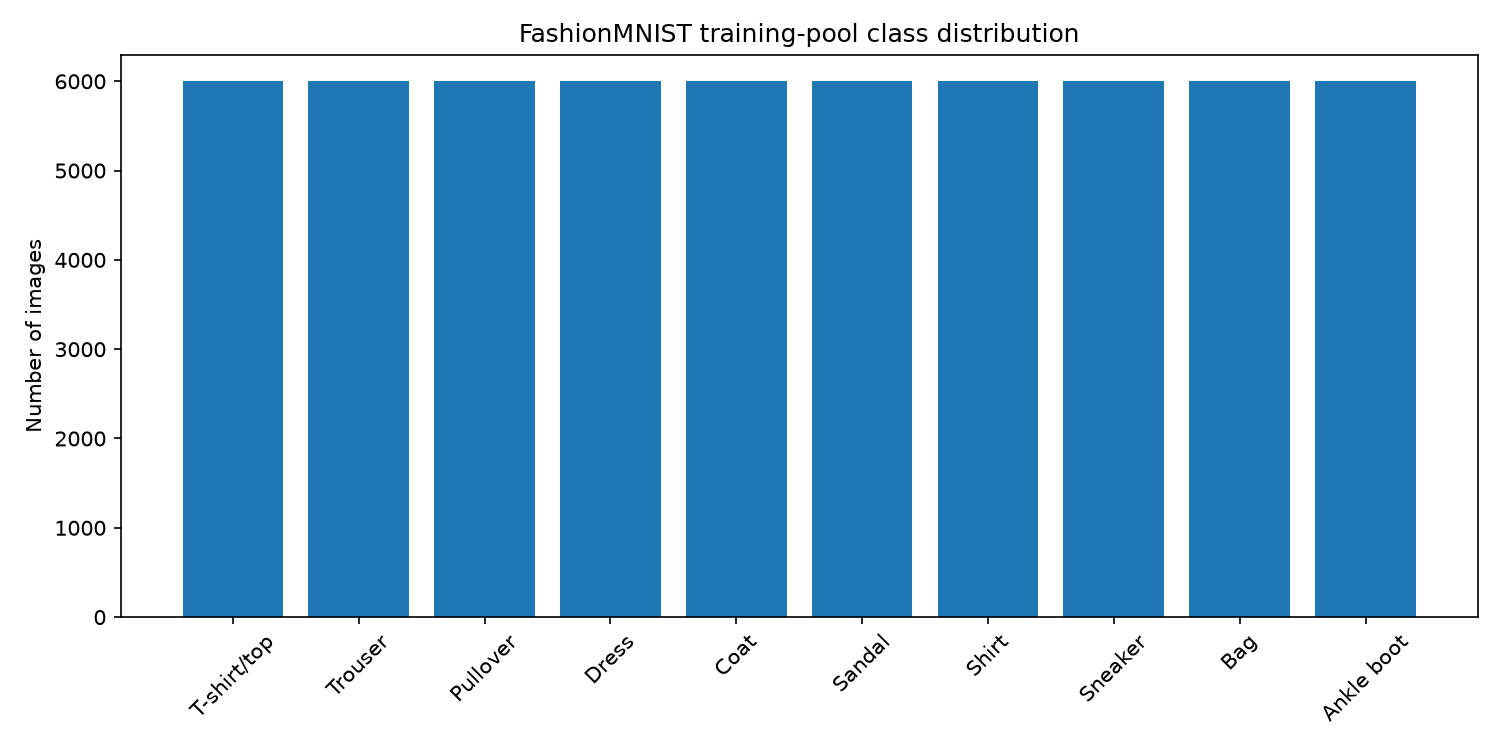
\includegraphics[width=0.9\textwidth]{../../Assignment1/outputs/eda/class_distribution.png}
    \caption{Fashion-MNIST training-pool class distribution.}
    \label{fig:eda-class-distribution}
\end{figure}

The class distribution is perfectly balanced, with 6,000 images for each of the ten classes in the official training pool. This balance reduces the risk that the classifiers are dominated by a majority class.

\begin{figure}[H]
    \centering
    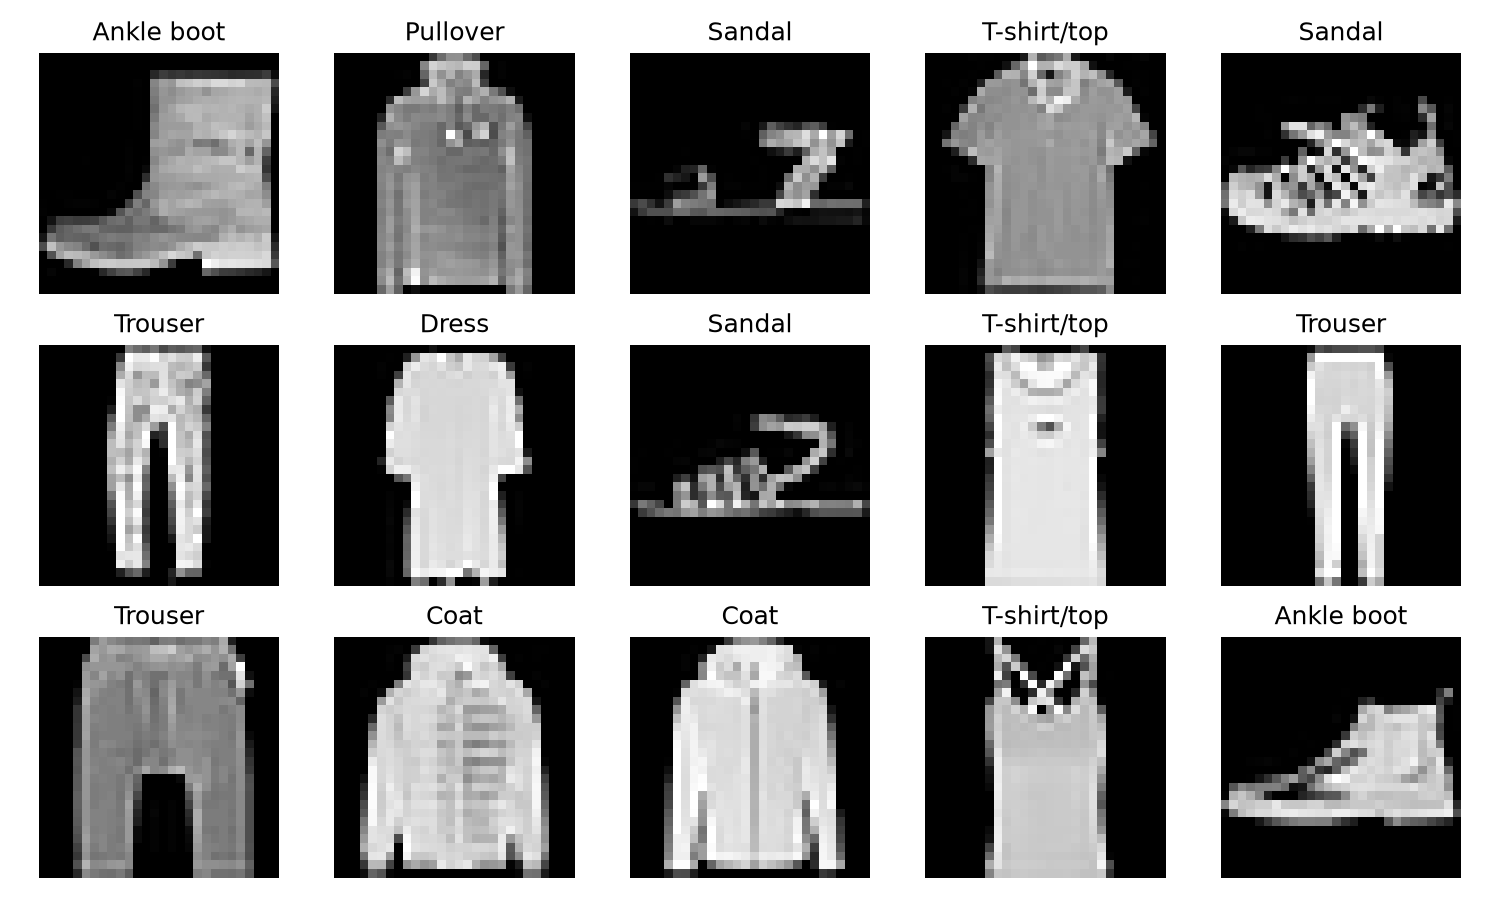
\includegraphics[width=0.9\textwidth]{../../Assignment1/outputs/eda/random_examples.png}
    \caption{Reproducibly selected Fashion-MNIST training examples.}
    \label{fig:eda-random-examples}
\end{figure}

The sampled images confirm that the dataset contains centered grayscale clothing objects with visually meaningful class labels. They also illustrate within-class variation in pose, shape, and intensity, which motivates using both a linear baseline and a nonlinear MLP model.

\begin{table}[H]
    \centering
    \caption{EDA statistics.}
    \label{tab:eda-statistics}
    \begin{tabular}{@{}lrr@{}}
        \toprule
        Statistic & Value & Notes \\
        \midrule
        Mean & 0.2860 & Computed on training-pool pixels scaled to $[0,1]$. \\
        Standard deviation & 0.3530 & Computed on training-pool pixels scaled to $[0,1]$. \\
        Minimum / maximum & 0.0 / 1.0 & Raw pixel values after scaling. \\
        Missing or invalid values & 0 detected & No missing-value handling was required. \\
        \bottomrule
    \end{tabular}
\end{table}

The images are represented as $1\times28\times28$ tensors with pixel values in $[0,1]$. The mean and standard deviation provide the normalization values used by the data-loading pipeline.

\subsection{Task-Specific EDA (Classification)}

For the classification task, the EDA additionally examines the geometry of the image representations and the similarity between class-level average images.

\begin{figure}[H]
    \centering
    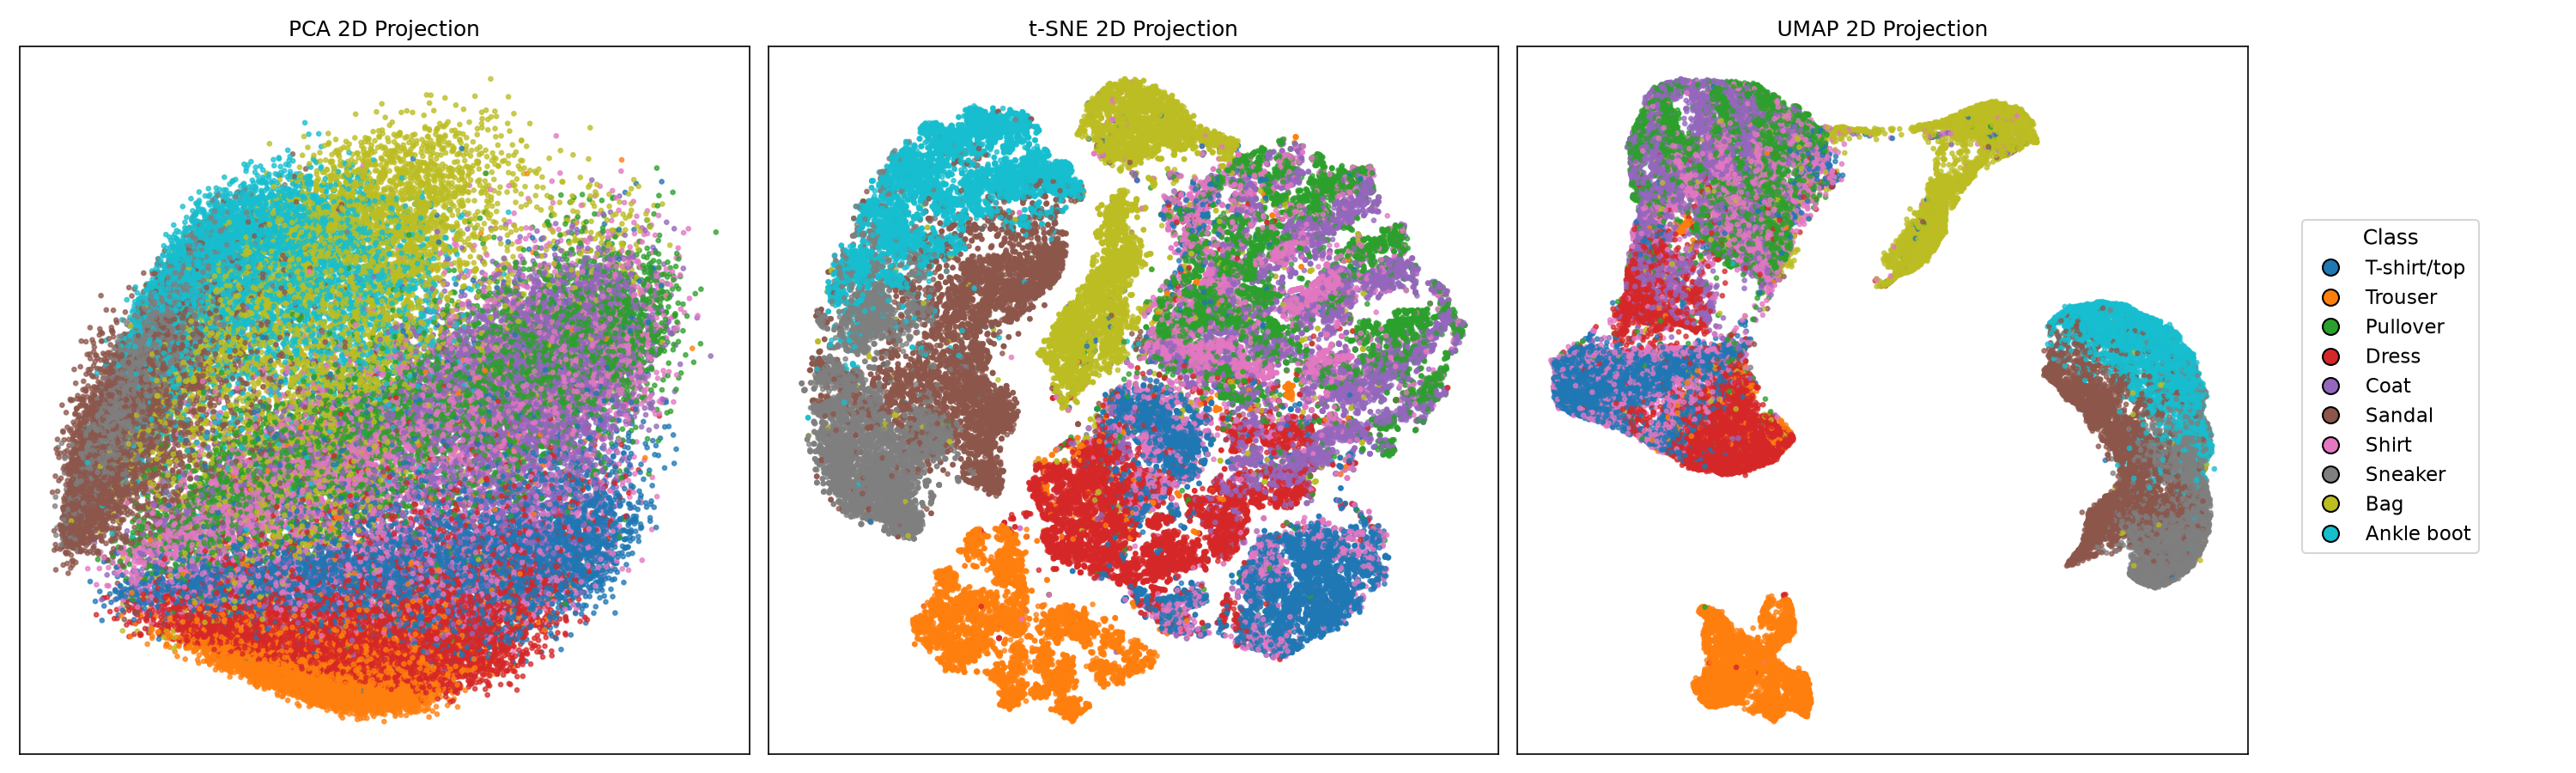
\includegraphics[width=\textwidth]{../../Assignment1/outputs/eda/dimensionality_reduction.png}
    \caption{PCA, t-SNE, and UMAP projections of sampled Fashion-MNIST images.}
    \label{fig:eda-dimensionality-reduction}
\end{figure}

The dimensionality-reduction views show that some classes form relatively coherent groups, while visually similar clothing categories overlap. PCA provides a broad linear view, whereas t-SNE and UMAP reveal more localized nonlinear structure. These projections suggest that footwear classes are often easier to separate, while upper-body categories may require more expressive decision boundaries.

\begin{figure}[H]
    \centering
    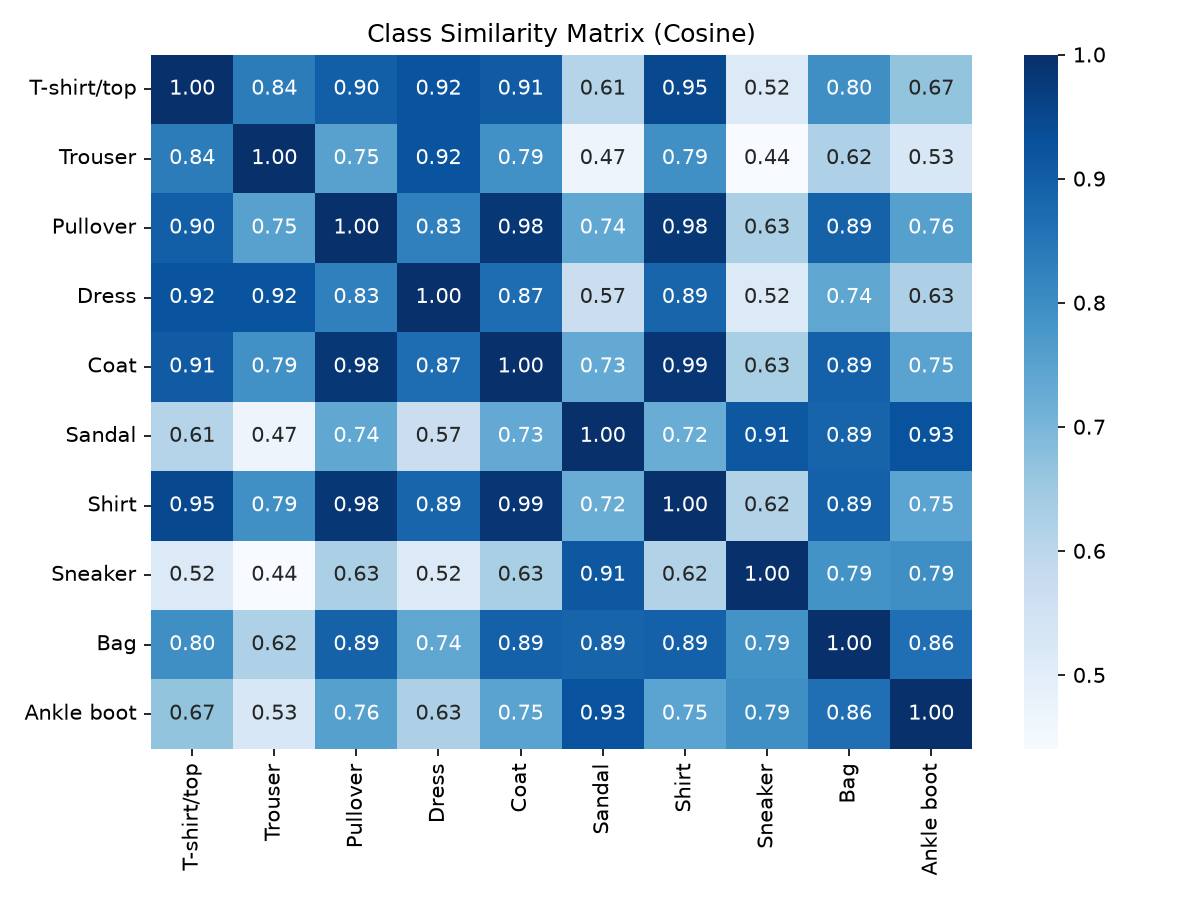
\includegraphics[width=0.78\textwidth]{../../Assignment1/outputs/eda/class_similarity_matrix.png}
    \caption{Cosine similarity between class-level mean images.}
    \label{fig:eda-class-similarity}
\end{figure}

The cosine-similarity matrix highlights pairs of classes with similar average visual structure. For example, Pullover--Coat and Coat--Shirt have high similarity, while Sandal--Trouser and Sneaker--Trouser are less similar. The high similarity among several upper-body classes indicates likely confusion regions for classification and motivates the later error analysis.
